% Generated by pysimcount.pffig13ext -- do not edit; regenerate instead.
% figure: fig13ext-cnot-lines-before -- Fig. 13 extended, CNOT, without Lie-Trotter S1, Suzuki S2, Suzuki S8; before optimisation only (diamonds)
% metric=cnot gatebase=cz unmerged; r_method=measured-fit: r = ceil(a n^b) fitted to measured r, mean over seeds [1, 2, 3, 4, 5, 6, 7, 8, 9, 10], n = [5, 6, 7, 8, 9, 10, 11]; every point extrapolated; y axis autoscaled (not the replica's range)
% optimised = Light reconstruction r x marginal + edge; verified n <= 16
% figure made at git_commit=3f419fd078cbd27a6e57919468bd4e5f1b96c08b git_dirty=False
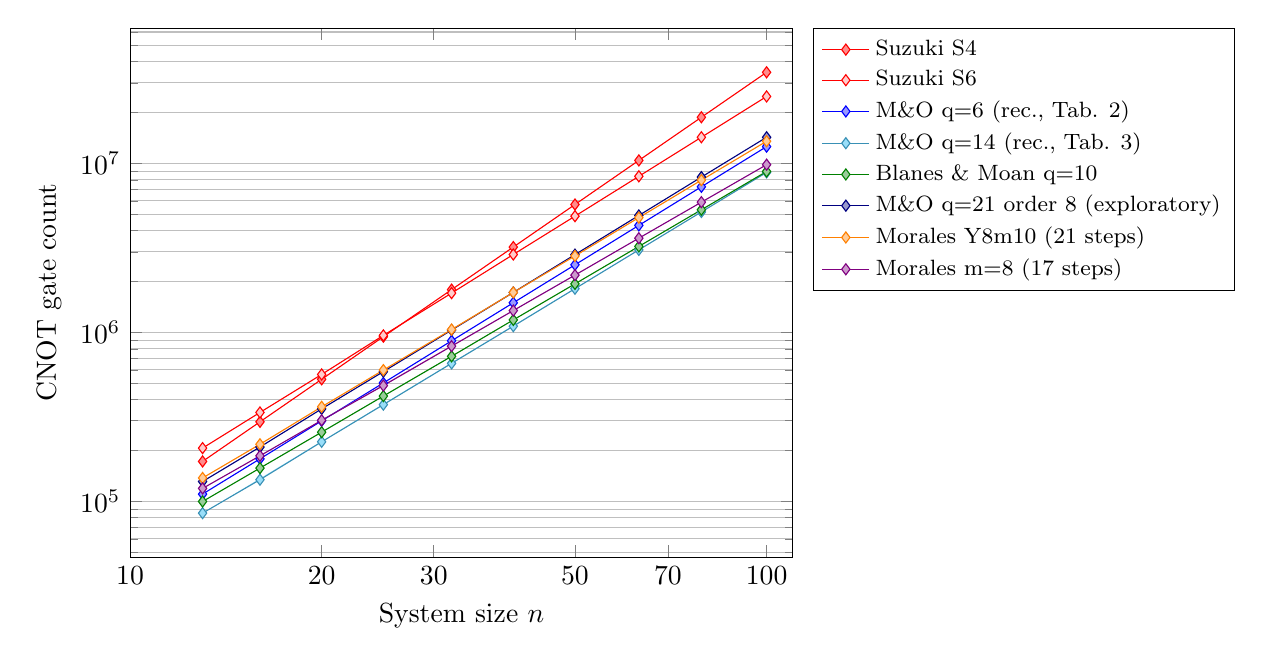
\begin{tikzpicture}
  \begin{loglogaxis}[
    width=10cm, height=8.3cm,
    xlabel={System size $n$}, ylabel={CNOT gate count},
    xmin=10, xmax=110,
    xtick={10,20,30,50,70,100}, xticklabels={10,20,30,50,70,100},
    ymajorgrids=true, yminorgrids=true,
    legend pos=outer north east, legend cell align=left,
    legend style={font=\footnotesize},
  ]
    \addplot[solid, mark=diamond*, mark size=2pt, draw=red, fill=red!45] coordinates {
      (13,172380)
      (16,295680)
      (20,528000)
      (25,943500)
      (32,1791360)
      (40,3199200)
      (50,5715000)
      (63,10421460)
      (79,18765660)
      (100,34626000)
    };
    \addlegendentry{Suzuki S4}
    \addplot[solid, mark=diamond*, mark size=2pt, draw=red, fill=red!20] coordinates {
      (13,206700)
      (16,336000)
      (20,564000)
      (25,960000)
      (32,1708800)
      (40,2892000)
      (50,4875000)
      (63,8391600)
      (79,14291100)
      (100,24900000)
    };
    \addlegendentry{Suzuki S6}
    \addplot[solid, mark=diamond*, mark size=2pt, draw=blue, fill=blue!40] coordinates {
      (13,110448)
      (16,178560)
      (20,299520)
      (25,502200)
      (32,891648)
      (40,1497600)
      (50,2512800)
      (63,4300128)
      (79,7274952)
      (100,12578400)
    };
    \addlegendentry{M\&O q=6 (rec., Tab. 2)}
    \addplot[solid, mark=diamond*, mark size=2pt, draw=cyan!70!black, fill=cyan!40] coordinates {
      (13,85176)
      (16,134400)
      (20,225120)
      (25,373800)
      (32,655872)
      (40,1088640)
      (50,1814400)
      (63,3079944)
      (79,5162808)
      (100,8853600)
    };
    \addlegendentry{M\&O q=14 (rec., Tab. 3)}
    \addplot[solid, mark=diamond*, mark size=2pt, draw=green!50!black, fill=green!50!black!40] coordinates {
      (13,99840)
      (16,157440)
      (20,256800)
      (25,420000)
      (32,721920)
      (40,1185600)
      (50,1938000)
      (63,3228120)
      (79,5318280)
      (100,8964000)
    };
    \addlegendentry{Blanes \& Moan q=10}
    \addplot[solid, mark=diamond*, mark size=2pt, draw=blue!50!black, fill=blue!50!black!40] coordinates {
      (13,131040)
      (16,209664)
      (20,352800)
      (25,585900)
      (32,1032192)
      (40,1723680)
      (50,2885400)
      (63,4921560)
      (79,8301636)
      (100,14288400)
    };
    \addlegendentry{M\&O q=21 order 8 (exploratory)}
    \addplot[solid, mark=diamond*, mark size=2pt, draw=orange, fill=orange!40] coordinates {
      (13,137592)
      (16,217728)
      (20,362880)
      (25,598500)
      (32,1040256)
      (40,1723680)
      (50,2835000)
      (63,4778676)
      (79,7963200)
      (100,13532400)
    };
    \addlegendentry{Morales Y8m10 (21 steps)}
    \addplot[solid, mark=diamond*, mark size=2pt, draw=violet, fill=violet!40] coordinates {
      (13,119340)
      (16,186048)
      (20,301920)
      (25,484500)
      (32,829056)
      (40,1346400)
      (50,2182800)
      (63,3611412)
      (79,5898456)
      (100,9832800)
    };
    \addlegendentry{Morales m=8 (17 steps)}
  \end{loglogaxis}
\end{tikzpicture}
